\documentclass[border=10pt]{standalone}
\usepackage{tikz}
\usepackage{makecell}

\tikzstyle{vertex}=[circle,draw,fill=black!20,minimum size=0.2cm,inner sep=0pt]
\tikzstyle{selected vertex} = [vertex, fill=blue!50]
\tikzstyle{edge} = [draw,thick,-]
\tikzstyle{weight} = [font=\small]
\tikzstyle{selected edge} = [draw,line width=3pt,-,red!50, opacity=0.5]
\tikzstyle{ignored edge} = [draw,line width=5pt,-,black!20]
\tikzstyle{text} = [text width=0.5cm]

\begin{document}
\noindent
    \centering
    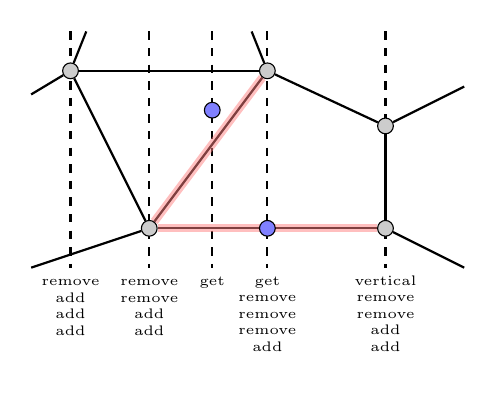
\begin{tikzpicture}[scale=1.0,transform shape,auto,swap]
		\path[edge, dashed] (-0, 2.5) -- (0, -0.5);
		\path[edge, dashed] (-1.5, 2.5) -- (-1.5, -0.5);
		\path[edge, dashed] (-2.2, 2.5) -- (-2.2, -0.5);
		\path[edge, dashed] (-3, 2.5) -- (-3, -0.5);
		\path[edge, dashed] (-4, 2.5) -- (-4, -0.5);
        \node[vertex] (1) at (0, 0) {};
        \node[vertex] (2) at (0, 1.3) {};
        \node[vertex] (3) at (-1.5, 2) {};
        \node[vertex] (4) at (-3, 0) {};
        \node[vertex] (5) at (-4, 2) {};
        \path[edge] (1) -- node[weight] {} (2);
        \path[edge] (1) -- node[weight] {} (4);
        \path[edge] (2) -- node[weight] {} (3);
        \path[edge] (3) -- node[weight] {} (4);
        \path[edge] (1) -- node[weight] {} (1, -0.5);
        \path[edge] (2) -- node[weight] {} (1, 1.8);
        \path[edge] (3) -- node[weight] {} (-1.7, 2.5);
        \path[edge] (3) -- node[weight] {} (5);
        \path[edge] (4) -- node[weight] {} (5);
        \path[edge] (4) -- node[weight] {} (-4.5, -0.5);
        \path[edge] (5) -- node[weight] {} (-3.8, 2.5);
        \path[edge] (5) -- node[weight] {} (-4.5, 1.7);
        \path[selected edge] (1) -- node[weight] {} (4);
        \path[selected edge] (3) -- node[weight] {} (4);
        \node[selected vertex] (6) at (-1.5, 0) {};
        \node[selected vertex] (7) at (-2.2, 1.5) {};
		\node[] at (-4, -1) {\tiny \makecell{remove\\add\\add\\add}};
		\node[] at (-3, -1) {\tiny \makecell{remove\\remove\\add\\add}};
		\node[] at (-2.2, -0.9) {\tiny \makecell{get\\ \\ \\}};
		\node[] at (-1.5, -1.1) {\tiny \makecell{get\\remove\\remove\\remove\\add}};
		\node[] at (0, -1.1) {\tiny \makecell{vertical\\remove\\remove\\add\\add}};
	\end{tikzpicture}
\end{document}
